For this case, the numerical simulation is performed for a real 
coronary artery with atherosclerosis whose geometry was obtained 
through an image processing as suggested by Wang et al. (2017) 
\cite{wang2017}. This geometry is particular to each patient 
due to the patient health conditions. As in the previous cases, 
an channel obstruction of 40\% was considered due to atherosclerosis 
and the stent strut was modeled by
10 uniformly spaced semi-circles.
The domain was discretized using 11807 nodes and 26426 linear 
triangular elements. 

\medskip
The \ref{velocity evolution real stent} shows the unsteady velocity 
profile in the position where the horizontal velocity 
has the maximum non-dimensional value ($x=6.65R$). 
As we can see, the maximum non-dimensional value of the velocity field 
reaches $u=3.68$ when the stent is placed. 
However, this velocity may vary according to the 
coronary artery geometry for each patient.

\begin{figure}[H]
     \centering
     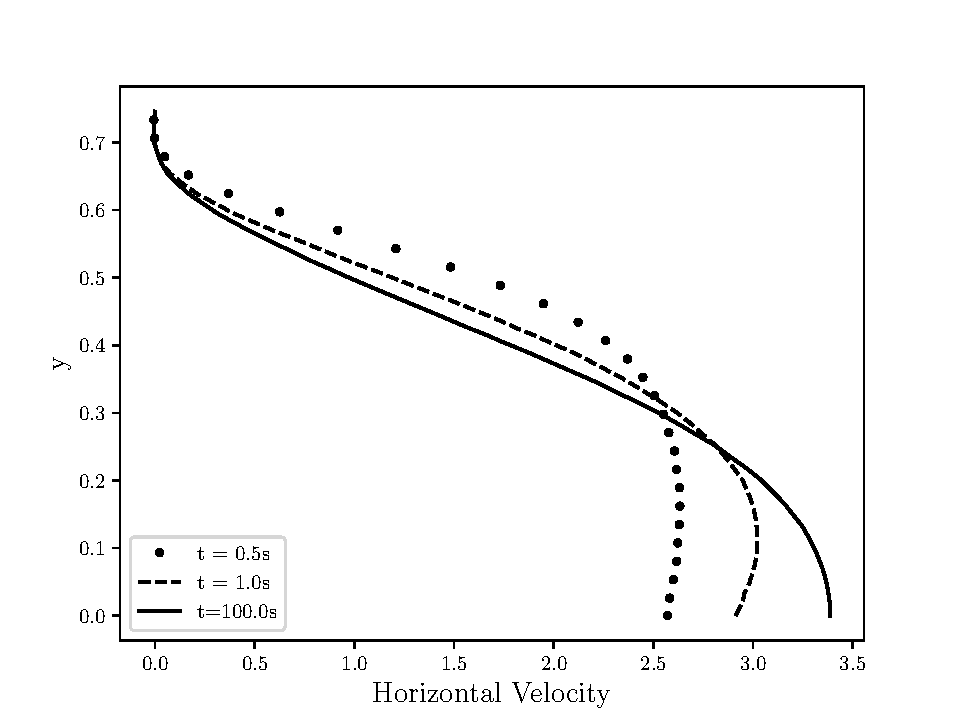
\includegraphics[scale=1]{./02_chaps/cap_solution/figure/vel_RealStrut_evol.pdf}\\
     \caption{
The unsteady velocity profile for real channel with drug-eluting stent.}
     \label{velocity evolution real stent}
\end{figure}

\newpage
The \ref{velocity field real stent} presents the evolution in 
time and space of the velocity field for half of the domain. 
The velocity field is represented with non-dimensional values 
where the red color refers to the $u=3.68$ value and the blue color 
$u=0$ value. Conveting to dimensional values, 
we have $u=44.2cm/s$ and $u=0cm/s$ respectively.


\vspace{2cm} 
\begin{figure}[H]
     \begin{minipage}{.50\linewidth}
      \centering
      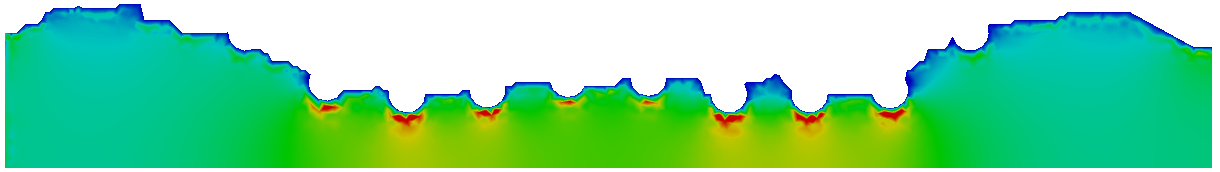
\includegraphics[scale=0.18]{./02_chaps/cap_solution/figure/vel_RealStrut1.png}\\
      t = 0.1
     \end{minipage}%
     \begin{minipage}{.50\linewidth}
      \centering
      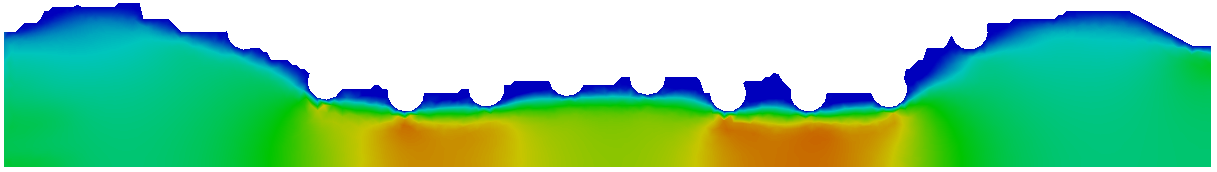
\includegraphics[scale=0.18]{./02_chaps/cap_solution/figure/vel_RealStrut2.png}\\
      t = 0.5
     \end{minipage}
     \begin{minipage}{.50\linewidth}
     \medskip
      \centering
      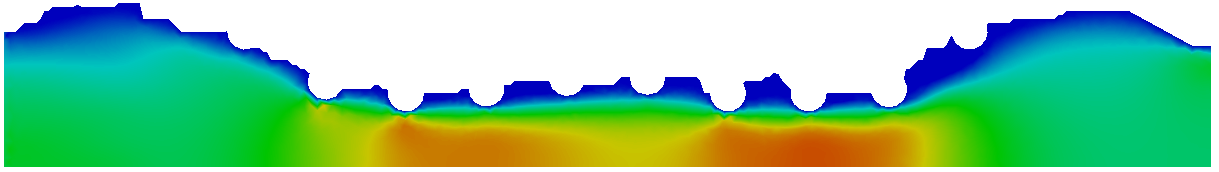
\includegraphics[scale=0.18]{./02_chaps/cap_solution/figure/vel_RealStrut3.png}\\
      t = 1.0
     \end{minipage}%
     \begin{minipage}{.50\linewidth}
     \medskip
      \centering
      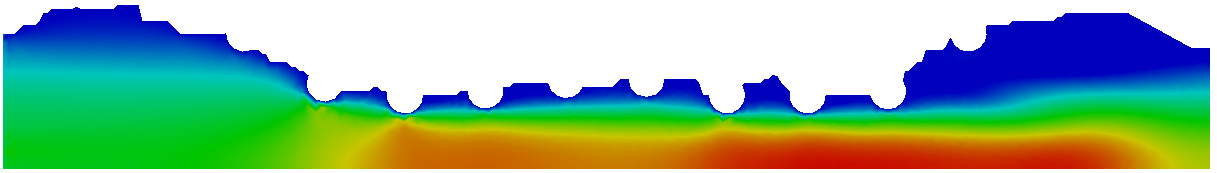
\includegraphics[scale=0.18]{./02_chaps/cap_solution/figure/vel_RealStrut4.png}\\
      t = 3.0
     \end{minipage}
     \begin{minipage}{.50\linewidth}
      \centering
      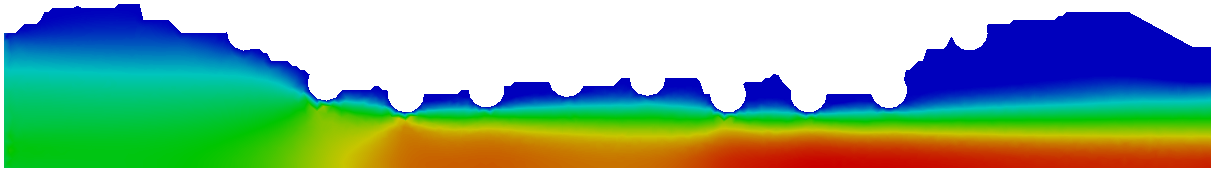
\includegraphics[scale=0.18]{./02_chaps/cap_solution/figure/vel_RealStrut5.png}\\
      t = 5.0
     \end{minipage}%
     \begin{minipage}{.50\linewidth}
      \centering
      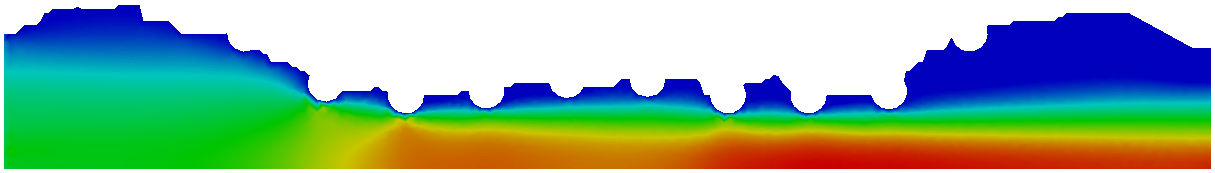
\includegraphics[scale=0.18]{./02_chaps/cap_solution/figure/vel_RealStrut6.png}\\
      t = 7.0
     \end{minipage}
     \begin{minipage}{.50\linewidth}
     \medskip
      \centering
      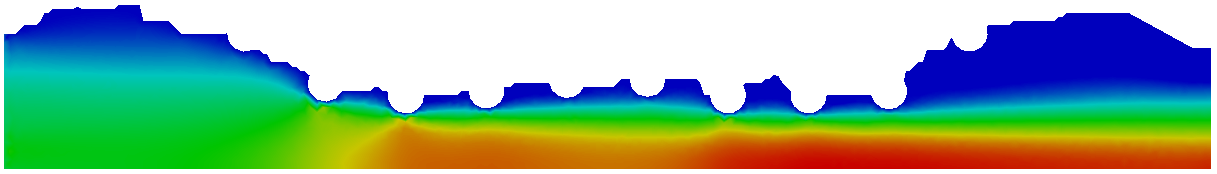
\includegraphics[scale=0.18]{./02_chaps/cap_solution/figure/vel_RealStrut7.png}\\
      t = 10.0
     \end{minipage}%
     \begin{minipage}{.50\linewidth}
     \medskip
      \centering
      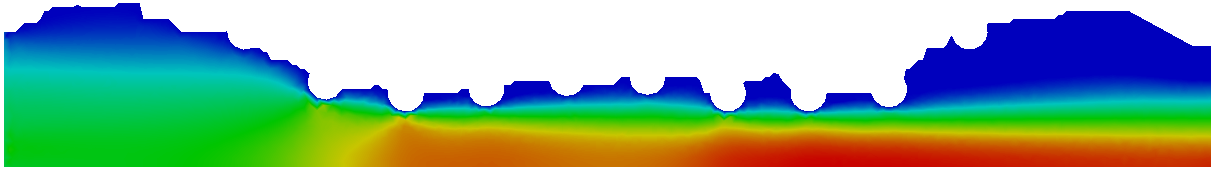
\includegraphics[scale=0.18]{./02_chaps/cap_solution/figure/vel_RealStrut8.png}\\
      steady state
     \end{minipage}\\[10pt]
      \centering
      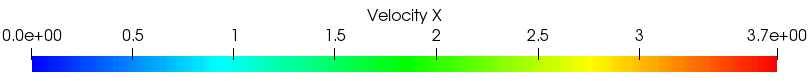
\includegraphics[scale=0.5]{./02_chaps/cap_solution/figure/vel_RealStrutScale.png}\\
     \medskip
     \caption{
Time and space evolution of the velocity field for real channel with
drug-eluting stent.}
     \label{velocity field real stent}
\end{figure}





\vspace{1cm}
The \ref{conc field real stent sc 1} and 
\ref{conc field real stent sc 10} show the time and space evolution 
of the concentration field for several \textit{Schmidt} number, 
such as: $1$, $10$, $100$ and $1000$ respectively. The concentration field is 
represented with the non-dimensional values where the red color 
represents $100$\% and the blue color represents $0$\% 
of the diffused concentration in the bloodstream. 
It is possible to observe that the \textit{Schmidt} number directly 
influences the drug transport in the blood flow. 
For high values of the \textit{Schmidt} number, 
the transport of chemical species becomes purely convective.


\begin{figure}[H]
     \begin{minipage}{.50\linewidth}
      \centering
      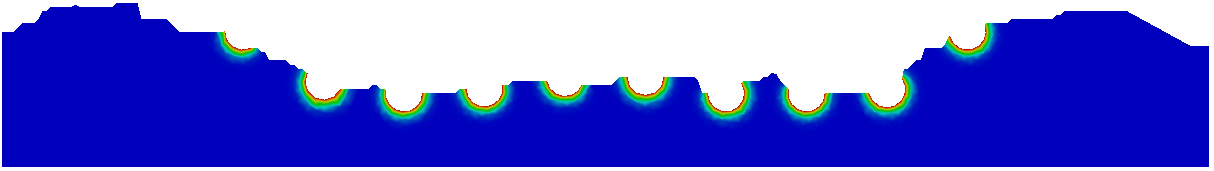
\includegraphics[scale=0.18]{./02_chaps/cap_solution/figure/conc1_RealStrut1.png}\\
      t = 0.1
     \end{minipage}%
     \begin{minipage}{.50\linewidth}
      \centering
      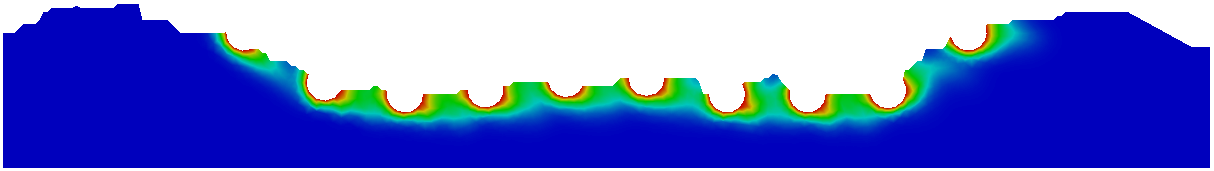
\includegraphics[scale=0.18]{./02_chaps/cap_solution/figure/conc1_RealStrut2.png}\\
      t = 0.5
     \end{minipage}
     \begin{minipage}{.50\linewidth}
     \medskip
      \centering
      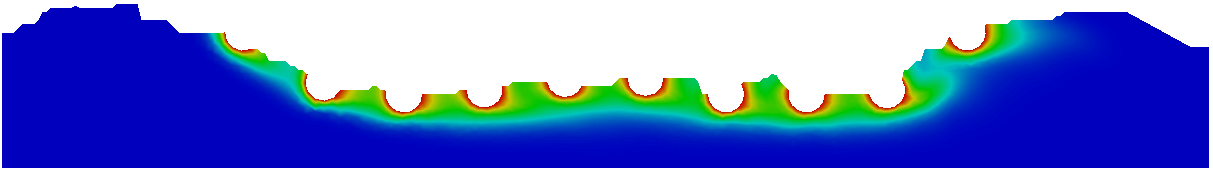
\includegraphics[scale=0.18]{./02_chaps/cap_solution/figure/conc1_RealStrut3.png}\\
      t = 1.0
     \end{minipage}%
     \begin{minipage}{.50\linewidth}
     \medskip
      \centering
      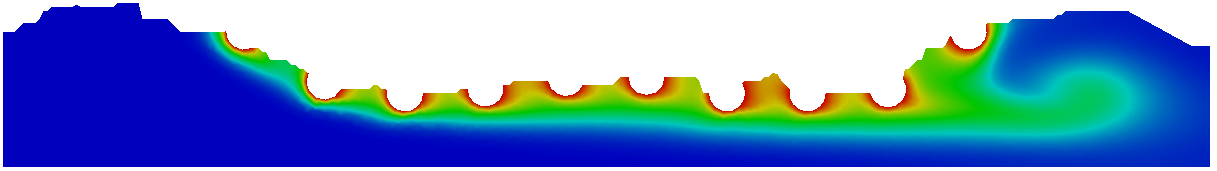
\includegraphics[scale=0.18]{./02_chaps/cap_solution/figure/conc1_RealStrut4.png}\\
      t = 3.0
     \end{minipage}
     \begin{minipage}{.50\linewidth}
      \centering
      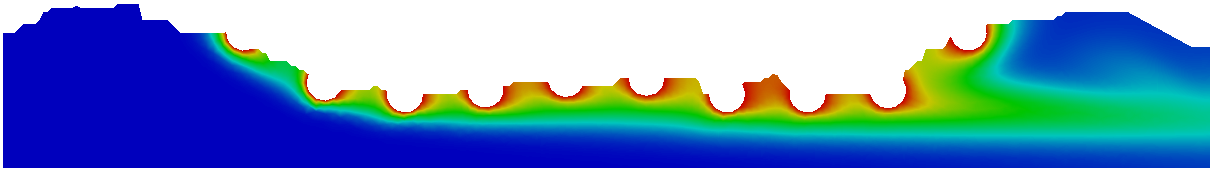
\includegraphics[scale=0.18]{./02_chaps/cap_solution/figure/conc1_RealStrut5.png}\\
      t = 5.0
     \end{minipage}%
     \begin{minipage}{.50\linewidth}
      \centering
      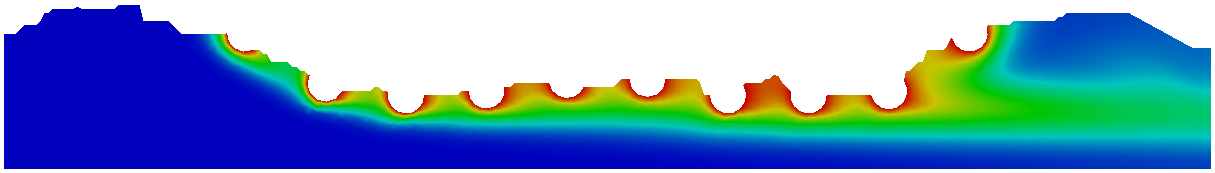
\includegraphics[scale=0.18]{./02_chaps/cap_solution/figure/conc1_RealStrut6.png}\\
      t = 7.0
     \end{minipage}
     \begin{minipage}{.50\linewidth}
     \medskip
      \centering
      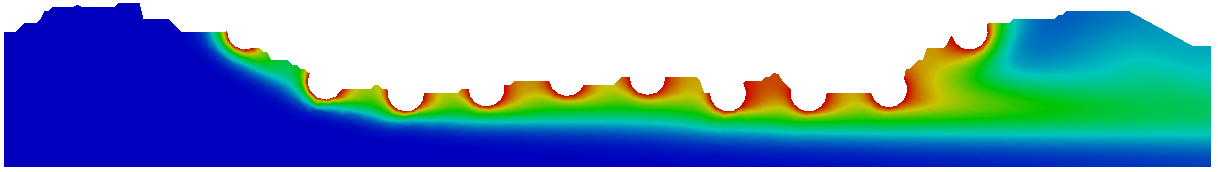
\includegraphics[scale=0.18]{./02_chaps/cap_solution/figure/conc1_RealStrut7.png}\\
      t = 10.0
     \end{minipage}%
     \begin{minipage}{.50\linewidth}
     \medskip
      \centering
      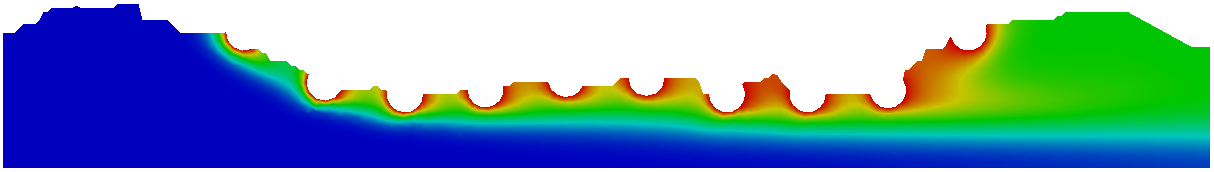
\includegraphics[scale=0.18]{./02_chaps/cap_solution/figure/conc1_RealStrut8.png}\\
      steady state
     \end{minipage}\\[10pt]
      \centering
      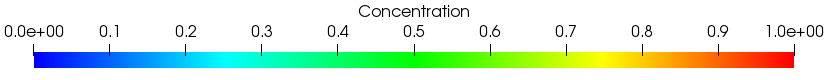
\includegraphics[scale=0.5]{./02_chaps/cap_solution/figure/conc1_RealStrutScale.png}\\
     \medskip
     \caption{
Time and space evolution of the concentration fiel for real channel with drug-eluting stent with $Sc=1$.}
     \label{conc field real stent sc 1}
\end{figure}



\begin{figure}[H]
     \begin{minipage}{.50\linewidth}
      \centering
      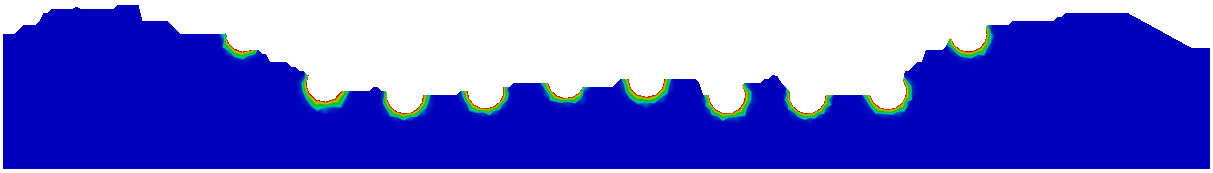
\includegraphics[scale=0.18]{./02_chaps/cap_solution/figure/conc10_RealStrut1.png}\\
      t = 0.1
     \end{minipage}%
     \begin{minipage}{.50\linewidth}
      \centering
      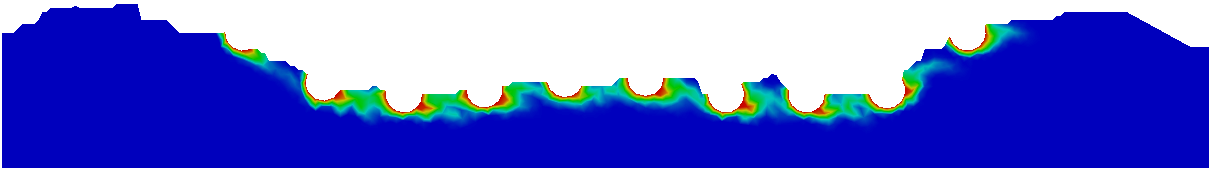
\includegraphics[scale=0.18]{./02_chaps/cap_solution/figure/conc10_RealStrut2.png}\\
      t = 0.5
     \end{minipage}
     \begin{minipage}{.50\linewidth}
     \medskip
      \centering
      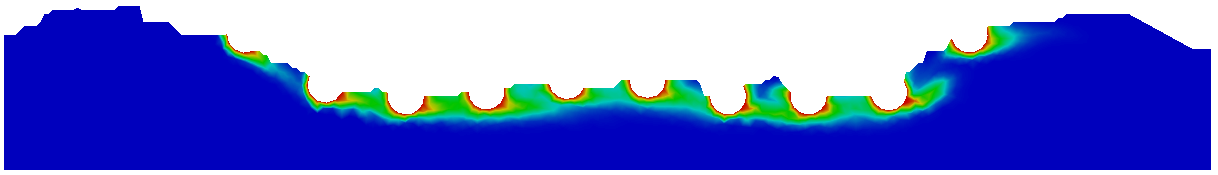
\includegraphics[scale=0.18]{./02_chaps/cap_solution/figure/conc10_RealStrut3.png}\\
      t = 1.0
     \end{minipage}%
     \begin{minipage}{.50\linewidth}
     \medskip
      \centering
      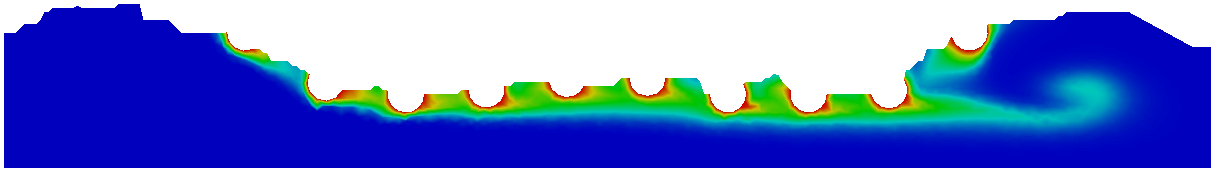
\includegraphics[scale=0.18]{./02_chaps/cap_solution/figure/conc10_RealStrut4.png}\\
      t = 3.0
     \end{minipage}
     \begin{minipage}{.50\linewidth}
      \centering
      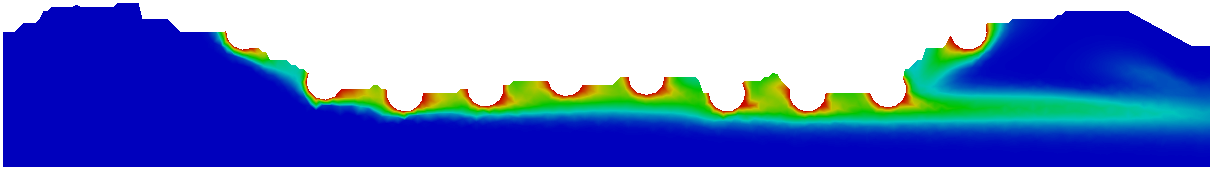
\includegraphics[scale=0.18]{./02_chaps/cap_solution/figure/conc10_RealStrut5.png}\\
      t = 5.0
     \end{minipage}%
     \begin{minipage}{.50\linewidth}
      \centering
      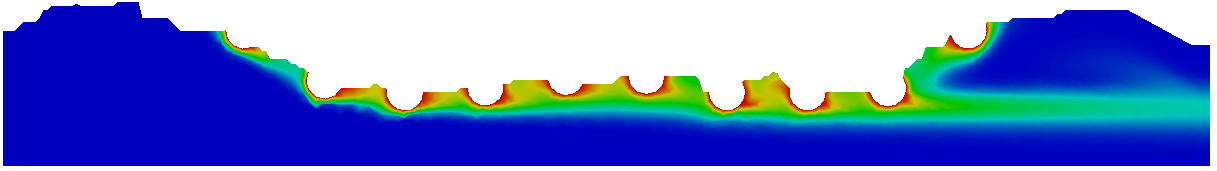
\includegraphics[scale=0.18]{./02_chaps/cap_solution/figure/conc10_RealStrut6.png}\\
      t = 7.0
     \end{minipage}
     \begin{minipage}{.50\linewidth}
     \medskip
      \centering
      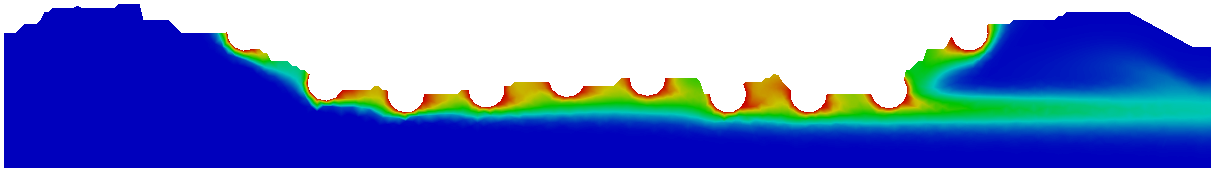
\includegraphics[scale=0.18]{./02_chaps/cap_solution/figure/conc10_RealStrut7.png}\\
      t = 10.0
     \end{minipage}%
     \begin{minipage}{.50\linewidth}
     \medskip
      \centering
      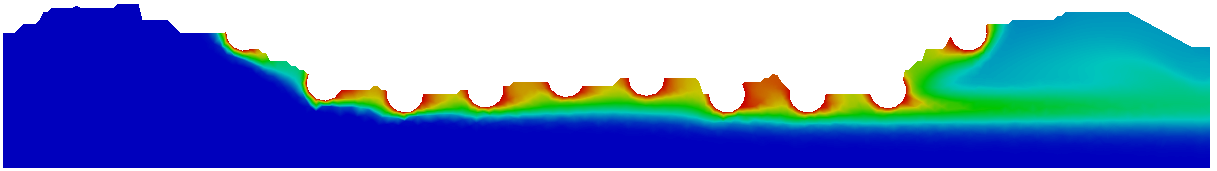
\includegraphics[scale=0.18]{./02_chaps/cap_solution/figure/conc10_RealStrut8.png}\\
      steady state
     \end{minipage}\\[10pt]
      \centering
      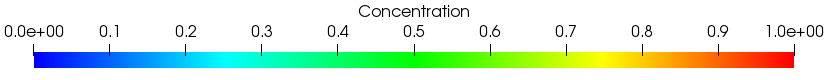
\includegraphics[scale=0.5]{./02_chaps/cap_solution/figure/conc1_RealStrutScale.png}\\
     \medskip
    \caption{
Time and space evolution of the concentration fiel for real channel with drug-eluting stent with $Sc=10$.}
     \label{conc field real stent sc 10}
\end{figure}



\begin{figure}[H]
     \begin{minipage}{.50\linewidth}
      \centering
      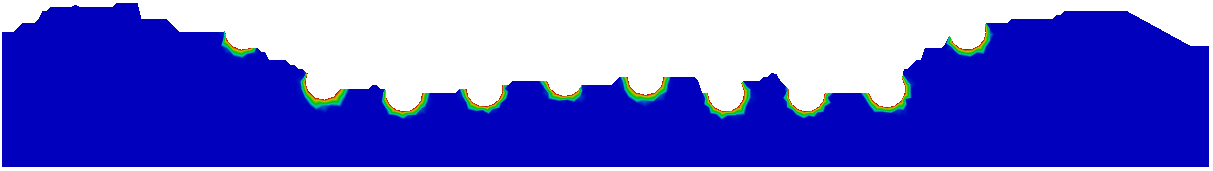
\includegraphics[scale=0.18]{./02_chaps/cap_solution/figure/conc100_RealStrut1.png}\\
      t = 0.1
     \end{minipage}%
     \begin{minipage}{.50\linewidth}
      \centering
      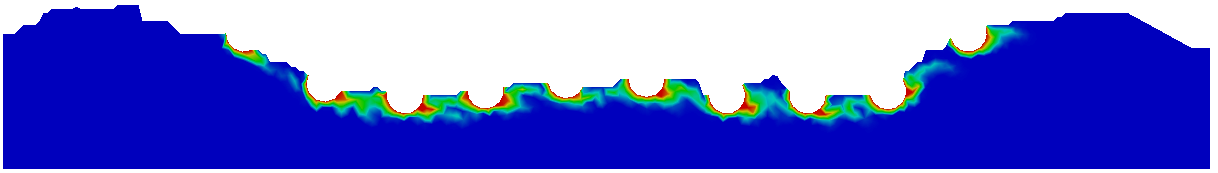
\includegraphics[scale=0.18]{./02_chaps/cap_solution/figure/conc100_RealStrut2.png}\\
      t = 0.5
     \end{minipage}
     \begin{minipage}{.50\linewidth}
     \medskip
      \centering
      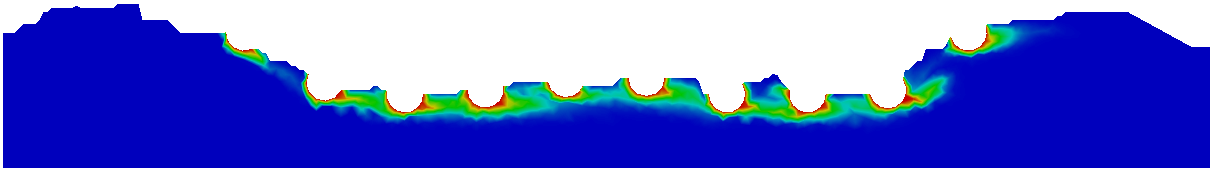
\includegraphics[scale=0.18]{./02_chaps/cap_solution/figure/conc100_RealStrut3.png}\\
      t = 1.0
     \end{minipage}%
     \begin{minipage}{.50\linewidth}
     \medskip
      \centering
      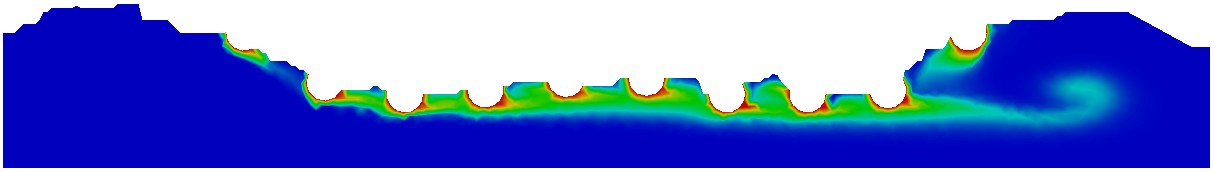
\includegraphics[scale=0.18]{./02_chaps/cap_solution/figure/conc100_RealStrut4.png}\\
      t = 3.0
     \end{minipage}
     \begin{minipage}{.50\linewidth}
      \centering
      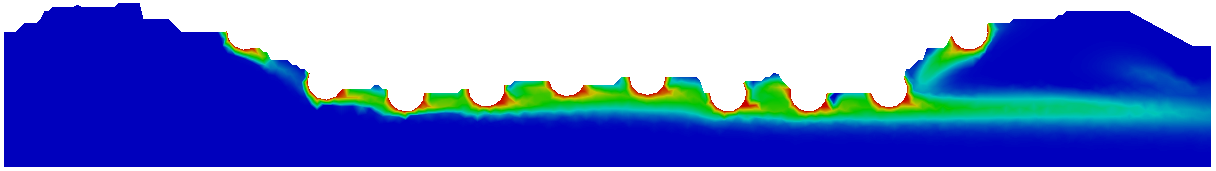
\includegraphics[scale=0.18]{./02_chaps/cap_solution/figure/conc100_RealStrut5.png}\\
      t = 5.0
     \end{minipage}%
     \begin{minipage}{.50\linewidth}
      \centering
      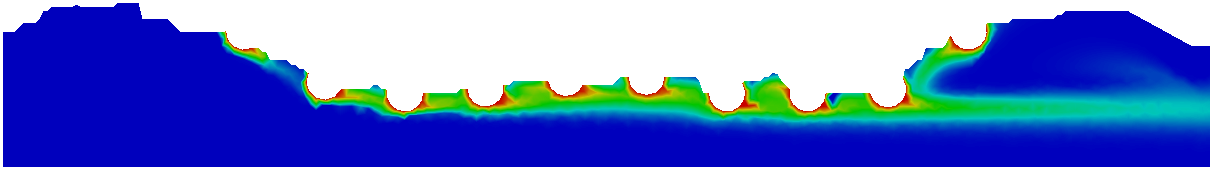
\includegraphics[scale=0.18]{./02_chaps/cap_solution/figure/conc100_RealStrut6.png}\\
      t = 7.0
     \end{minipage}
     \begin{minipage}{.50\linewidth}
     \medskip
      \centering
      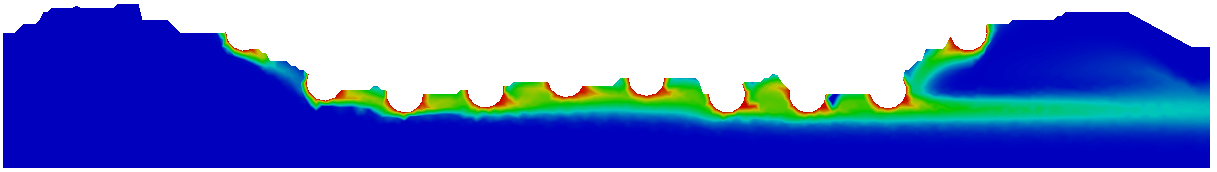
\includegraphics[scale=0.18]{./02_chaps/cap_solution/figure/conc100_RealStrut7.png}\\
      t = 10.0
     \end{minipage}%
     \begin{minipage}{.50\linewidth}
     \medskip
      \centering
      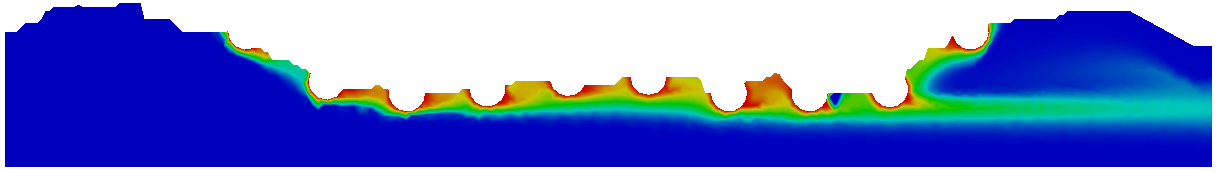
\includegraphics[scale=0.18]{./02_chaps/cap_solution/figure/conc100_RealStrut8.png}\\
      steady state
     \end{minipage}\\[10pt]
      \centering
      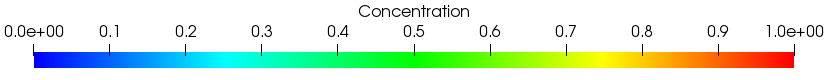
\includegraphics[scale=0.5]{./02_chaps/cap_solution/figure/conc1_RealStrutScale.png}\\
     \medskip
    \caption{
Time and space evolution of the concentration fiel for real channel with drug-eluting stent with $Sc=100$.}
     \label{conc field real stent sc 100}
\end{figure}


\begin{figure}[H]
     \begin{minipage}{.50\linewidth}
      \centering
      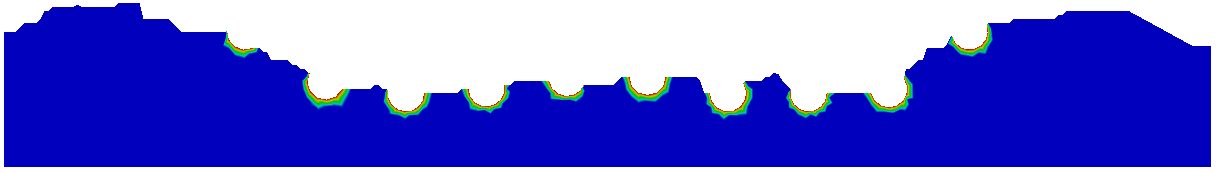
\includegraphics[scale=0.18]{./02_chaps/cap_solution/figure/conc1000_RealStrut1.png}\\
      t = 0.1
     \end{minipage}%
     \begin{minipage}{.50\linewidth}
      \centering
      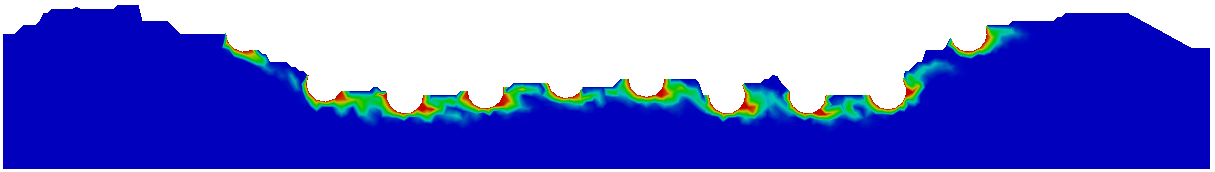
\includegraphics[scale=0.18]{./02_chaps/cap_solution/figure/conc1000_RealStrut2.png}\\
      t = 0.5
     \end{minipage}
     \begin{minipage}{.50\linewidth}
     \medskip
      \centering
      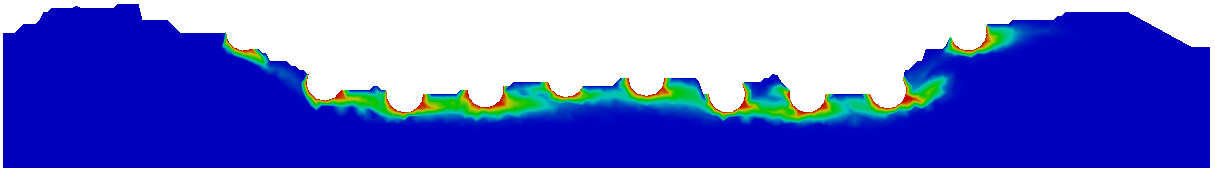
\includegraphics[scale=0.18]{./02_chaps/cap_solution/figure/conc1000_RealStrut3.png}\\
      t = 1.0
     \end{minipage}%
     \begin{minipage}{.50\linewidth}
     \medskip
      \centering
      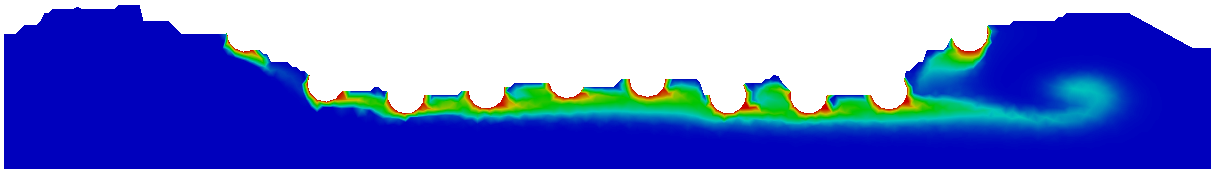
\includegraphics[scale=0.18]{./02_chaps/cap_solution/figure/conc1000_RealStrut4.png}\\
      t = 3.0
     \end{minipage}
     \begin{minipage}{.50\linewidth}
      \centering
      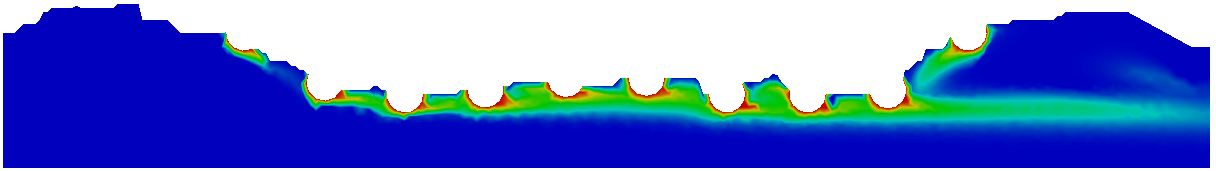
\includegraphics[scale=0.18]{./02_chaps/cap_solution/figure/conc1000_RealStrut5.png}\\
      t = 5.0
     \end{minipage}%
     \begin{minipage}{.50\linewidth}
      \centering
      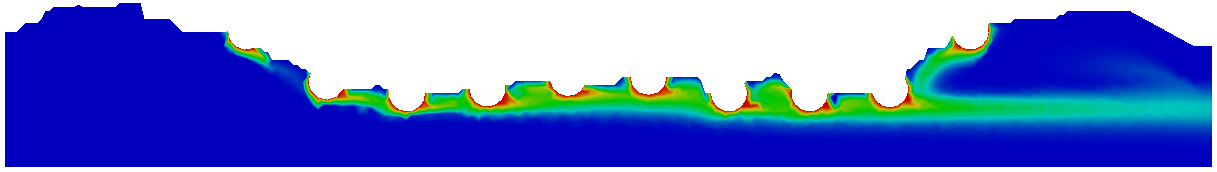
\includegraphics[scale=0.18]{./02_chaps/cap_solution/figure/conc1000_RealStrut6.png}\\
      t = 7.0
     \end{minipage}
     \begin{minipage}{.50\linewidth}
     \medskip
      \centering
      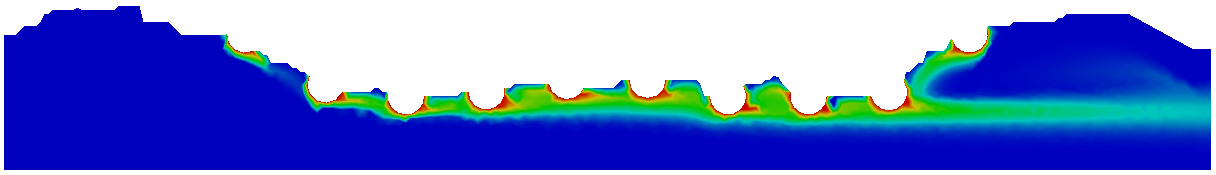
\includegraphics[scale=0.18]{./02_chaps/cap_solution/figure/conc1000_RealStrut7.png}\\
      t = 10.0
     \end{minipage}%
     \begin{minipage}{.50\linewidth}
     \medskip
      \centering
      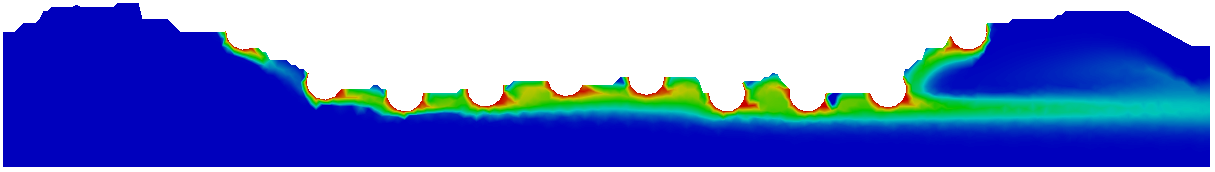
\includegraphics[scale=0.18]{./02_chaps/cap_solution/figure/conc1000_RealStrut8.png}\\
      steady state
     \end{minipage}\\[10pt]
      \centering
      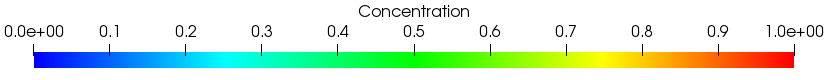
\includegraphics[scale=0.5]{./02_chaps/cap_solution/figure/conc1_RealStrutScale.png}\\
     \medskip
    \caption{
Time and space evolution of the concentration fiel for real channel with drug-eluting stent with $Sc=1000$.}
     \label{conc field real stent sc 1000}
\end{figure}




\newpage


